\documentclass{beamer}

\usepackage{tikz}
\usepackage{listings}
\usetikzlibrary{automata,positioning}
\usepackage{attrib}
\lstset{
basicstyle=\footnotesize \ttfamily,
language=Promela,
numbers=left,
xleftmargin=2em,
framexleftmargin=1.5em
}

\title{Model Checking}
\subtitle{Modeling concurrent systems and specification of correctness properties}
\author{Lukas Hofmaier \texttt{lukas.hofmaier@hsr.ch}}
\date{June 25, 2013 \\ Progam Analysis and Transformation Seminar FS13}

\begin{document}
\maketitle
\begin{frame}
  \frametitle{Outline}
  \tableofcontents
\end{frame}

\section{Model Checking}

\begin{frame}
  \frametitle{What's all about?}
  Does a behavioral model $S$ satisfy a defined property $P$?
  \[
  S \models P
  \]
  \begin{description}
  \item[S] Model written in Promela, describes the behavior of a system
  \item[$\models$] Satisfaction relation
  \item[P] Property to vefify, written in LTL notation
  \end{description}
\end{frame}

\begin{frame}
  \frametitle{Why Model Checking}
Alternate software verification techniques:
  \begin{description}
  \item[Peer review] Code is analyzed statically. Difficult to detect errors caused by concurrency.
  \item[Testing] Code is compiled and executed. Can expose error. Cannot proof absence of errors.
  \end{description}\
Model checking checks 100\% of all possible paths. But Model checking suffers from the state exposion problem.
\end{frame}

\section{Modeling Concurrent Systems}

\begin{frame}
  \frametitle{  Defining $S$ in $S \models P$}

  \begin{itemize}
  \item A model is written that describes the behavior (not the structure) of the system $S$.
  \item Spin checks verification models.
  \item The specification language that it accepts is called Promela.
  \item Emphasis of Promela is on modeling of process synchronization.
  \end{itemize}
\end{frame}

\subsection{Interleaving}



\begin{frame}[fragile]
  \frametitle{A first Mickey Mouse example}
  \begin{columns}
    \begin{column}{.5\textwidth}
    \begin{block}{Verification model}
      \begin{figure}
        \centering
\begin{lstlisting}
byte x=0;
active proctype A(){
       byte tempA = x + 2;
       x = tempA
}
\end{lstlisting}
      \end{figure}
    \end{block}
    \end{column}
    \begin{column}{.5\textwidth}
      \begin{block}{State diagram}
      \begin{figure}
        \centering
        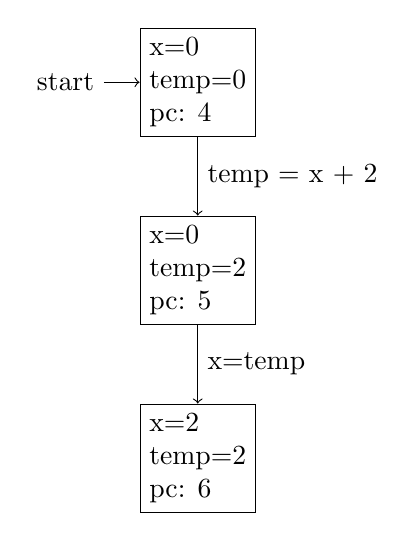
\begin{tikzpicture}[auto]
          \node[state, initial, rectangle, align=left](s1){x=0\\ temp=0\\pc: 4};
          \node[state, rectangle, align=left, below =of s1](s2){x=0\\temp=2\\pc: 5};
          \node[state, rectangle, align=left, below =of s2](s3){x=2\\temp=2\\pc: 6};
          \path[->](s1) edge node {temp = x + 2}(s2);
          \path[->](s2) edge node {x=temp}(s3);
        \end{tikzpicture}   
      \end{figure} 
      \end{block}
    \end{column}    
  \end{columns}
\end{frame}

\begin{frame}
  \frametitle{Interleaving}
  \begin{block}{Problem}
How does a state diagram of a system with several active processes look like?      \end{block}
\begin{block}{Arbitrarily interleaving}
  
\end{block}
  \begin{itemize}
  \item Interleaving is a paradigm to model systems with multiple processes.
  \item Based on the view that only one processor is available.
  \item A global state is composed of current individual states of all active processes.
  \item In every state non-deterministic choice between which state comes next.
  \item Program statements are interlocked.
  \item Interleaving is a enumeration of all possible state sequences.
  \end{itemize}
\end{frame}

\begin{frame}[fragile]
  \frametitle{System with two active processes}
  \lstinputlisting{interleavingproc.pml}
\end{frame}

\begin{frame}[fragile]
  \frametitle{Interleaved perspective}
  \begin{figure}
    \centering
    
\scalebox{0.8}{
   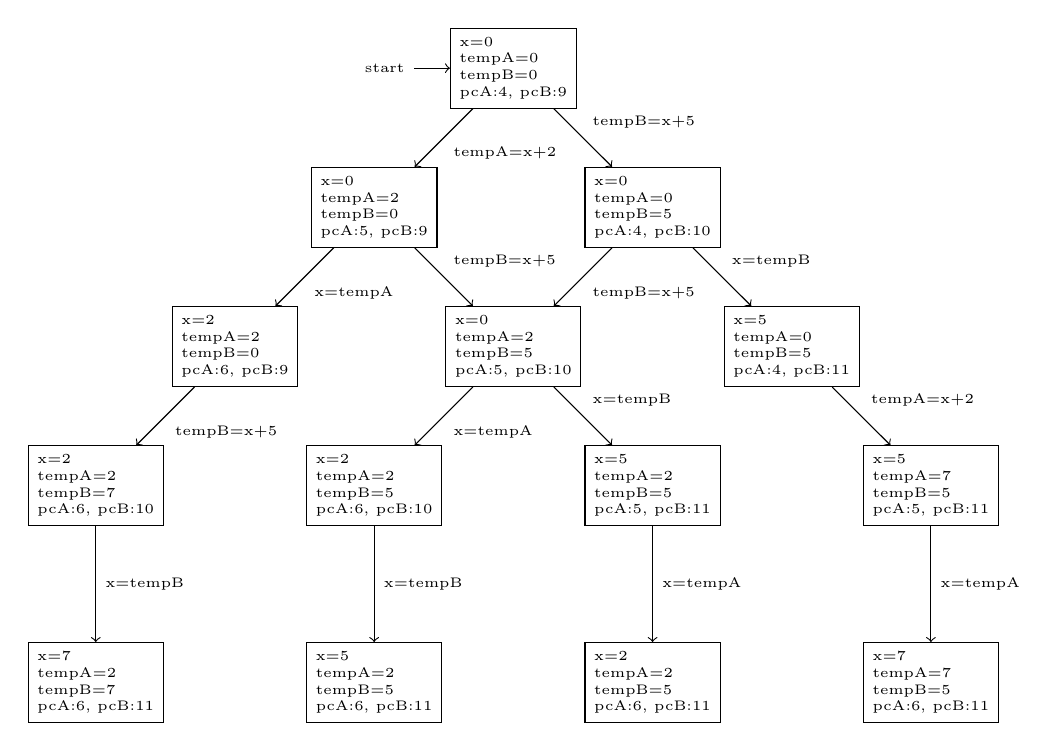
\begin{tikzpicture}[node distance=2.5cm, on grid, auto]
\tikzstyle{every node}=[font=\tiny]
   \node[state, initial, rectangle, align=left](s1){x=0\\tempA=0\\tempB=0\\pcA:4, pcB:9};
   \node[state, rectangle, align=left](s2) [below left=of s1]{x=0\\tempA=2\\tempB=0\\pcA:5, pcB:9};
   \node[state, rectangle, align=left](s3)[below left=of s2]{x=2\\tempA=2\\tempB=0\\pcA:6, pcB:9};
  \node[state, rectangle, align=left](s4)[below left=of s3]{x=2\\tempA=2\\tempB=7\\pcA:6, pcB:10};
\node[state, rectangle, align=left](s5)[below =of s4]{x=7\\tempA=2\\tempB=7\\pcA:6, pcB:11};
\node[state, rectangle, align=left](s6)[below right=of s1]{x=0\\tempA=0\\tempB=5\\pcA:4, pcB:10};
\node[state, rectangle, align=left](s7)[below right=of s6]{x=5\\tempA=0\\tempB=5\\pcA:4, pcB:11};
\node[state, rectangle, align=left](s8)[below right=of s7]{x=5\\tempA=7\\tempB=5\\pcA:5, pcB:11};
\node[state, rectangle, align=left](s9)[below =of s8]{x=7\\tempA=7\\tempB=5\\pcA:6, pcB:11};
\node[state, rectangle, align=left](s10)[below right=of s2]{x=0\\tempA=2\\tempB=5\\pcA:5, pcB:10};
\node[state, rectangle, align=left](s11)[below left=of s10]{x=2\\tempA=2\\tempB=5\\pcA:6, pcB:10};
\node[state, rectangle, align=left](s12)[below right=of s10]{x=5\\tempA=2\\tempB=5\\pcA:5, pcB:11};
\node[state,rectangle, align=left](s13)[below =of s11]{x=5\\tempA=2\\tempB=5\\pcA:6, pcB:11};
\node[state, rectangle, align=left](s14)[below =of s12]{x=2\\tempA=2\\tempB=5\\pcA:6, pcB:11};
   \path[->](s1) edge node {tempA=x+2}(s2);
   \path[->](s2) edge node {x=tempA}(s3);
   \path[->](s3) edge node {tempB=x+5}(s4);
\path[->](s4) edge node {x=tempB}(s5);
\path[->](s1) edge node {tempB=x+5}(s6);
\path[->](s6) edge node {x=tempB}(s7);
\path[->](s7) edge node {tempA=x+2}(s8);
\path[->](s8) edge node {x=tempA}(s9);
\path[->](s2) edge node {tempB=x+5}(s10);
\path[->](s6) edge node {tempB=x+5}(s10);
\path[->](s10) edge node {x=tempA}(s11);
\path[->](s10) edge node {x=tempB}(s12);
\path[->](s11) edge node {x=tempB}(s13);
\path[->](s12) edge node {x=tempA}(s14);
\end{tikzpicture}
}
\end{figure}

\end{frame}

\subsection{Synchronization}

\begin{frame}
  \frametitle{Synchronization Motivation}
  \begin{quote}
    Race conditions are a real nemesis that should be eliminated at the root. For an application that deals with mutability, every single access to shared mutable state must be verified to be correct. Even if one of them is broken, the entire application is broken. This is a tall order for our concurrent app to fall apart, only a single line of code that deals with concurrency needs to take a wrong step. In fact, a significant number of concurrent Java apps are broken, and we simply don’t know it.

 \attrib{ - Venkat Subramaniam \cite{subra11} -}
  \end{quote} 

\end{frame}

\begin{frame}[fragile]
  \frametitle{Lock the critical section with a mutex}
  \begin{figure}
    \centering
    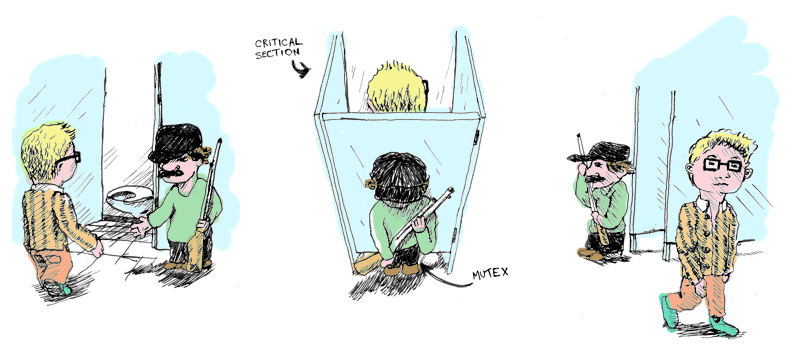
\includegraphics[scale=0.3]{mutex}
  \end{figure}
\begin{lstlisting}
#define acquire(mutex) atomic{mutex>0;mutex--;}
#define release(mutex) mutex++;
byte mutex=1
\end{lstlisting}

\end{frame}

\begin{frame}
  \frametitle{Locks are super tricky to use}
  \begin{figure}
    \centering
  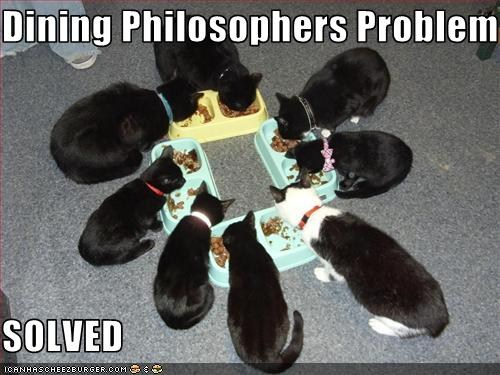
\includegraphics[scale=0.7]{dpsolved}
  \end{figure}
\end{frame}

\section{How to define correctness properties}

\begin{frame}
  \frametitle{Defining $P$ in $S \models P$}
  

\end{frame}

\subsection{Atomic propositions}


\begin{frame}[fragile]
  \frametitle{Atomic Propositions}
  \begin{itemize}
  \item Declarative sentences or expression. Can either be true or false.
  \item Evaluate to true or false
  \end{itemize}
  \begin{block}{Example}
\begin{lstlisting}
bool critA=0;
active proctype A(){
   critA = True;
   //critical section
   critA = False
}
\end{lstlisting}
The expression \texttt{(critA)} is an atomic proposition.
  \end{block}
\end{frame}

\subsection{Traces and words}

\begin{frame}
  \frametitle{Traces and words}
  Traces are an important concept to understand Linear-Time Properties.
  \begin{itemize}
  \item A computation is a sequence of states.
  \item Every state $s_i$ can be mapped to a subset of $2^{AP}$. $2^{AP}$ is the power set of $AP$.
  \item The subset contains a combination of atomic propositions that evaluate to true in the corresponding state.
  \item Multiple different sequences possible for the same system (non-determinism, different input) $\rightarrow$ several different traces.
  \item $\text{Traces}(S)$ represents all possible traces of system $S$.
  \end{itemize}
\end{frame}

\begin{frame}[fragile]
  \frametitle{Trace example}
  \begin{columns}
    \begin{column}{.4\textwidth}
      \begin{block}{Verification model}
        \begin{lstlisting}[frame=single]
bool critA=False;
bool critB=False;
proctype A(){
  critA = True;
  //critsec
  critA = False
}
proctype B(){
  critB = True;
  //critsec
  critB = False
}
\end{lstlisting}
      \end{block}
    \end{column}

    \begin{column}{.6\textwidth}
      \begin{block}{Possible sequence (of several possible)}
        \begin{equation*}
  \label{eq:path}
  \begin{split}
(4,9,critA=False,critB=False) \rightarrow \\
(6, 9, critA=True,critB=False) \rightarrow \\
(7, 9, critA=False,critB=False) \rightarrow \\
(7,11,critA=False,critB=True) \rightarrow \\
(7,12,critA=False,critB=False)
  \end{split}
\end{equation*}
      \end{block}
    \end{column}
  \end{columns}
\end{frame}

\begin{frame}
  \frametitle{Sequence $\rightarrow$ trace}
  \begin{block}{Sequence}
        \begin{equation*}
  \label{eq:path}
  \begin{split}
\pi=(4,9,critA=False,critB=False) \rightarrow \\
(6, 9, critA=True,critB=False) \rightarrow \\
(7, 9, critA=False,critB=False) \rightarrow \\
(7,11,critA=False,critB=True) \rightarrow \\
(7,12,critA=False,critB=False)
  \end{split}
\end{equation*}    
  \end{block}

  \begin{block}{Atomic propositions}
    \[
\text{AP}=\{critA, critB\}
\]
  \end{block}
  \begin{block}{Trace or word}
\[
trace(\pi) = \varnothing \{critA\} \varnothing \{critB\} \varnothing
\].
  \end{block}
\end{frame}
\subsection{Linear-Time Properties}

\begin{frame}
  \frametitle{Linear-Time Properties}
    \begin{description}
    \item[Linear-time] Concept where time is seen sequentially.
    \item[Linear-time property] Specify the traces that a system should exhibit. Defines a language over $2^{AP}$.
    \item[Traces($S$)] All traces or words that system accepts. Defines a language over $2^{AP}$.
    \end{description}
If $P$ is a Linear-time Property, then $S$ satisfies $P$, if $\text{Traces}(S) \subseteq P$. 
\[
TS \models P \iff \text{Traces}(S) \subseteq P 
\]

\end{frame}

\subsubsection{Safety properties}

\begin{frame}
  \frametitle{Claim mutual exlusion with $P_{mutex}$! }
  Now we can express the requirement of mutual exlusion.
  \begin{block}{For a single state}
\[
 \neg critA \lor \neg critB
\]
Evaluates to false if critA and critB are true.
  \end{block}
  \begin{block}{For $(2^{AP})^{\omega}$ - the set of all possible words in $2^{AP}$}
\[
P_{mutex}   = {A_0 A_1 A_2 \dots \in (2^{AP})^{\omega} | \forall i \geq 0.   A_i \models \neg critA \lor \neg critB}
\]
The language $P_{mutex}$ contains no words with $\{critA,critB\}$. $\{critA,critB\} \not \subseteq A_i$
  \end{block}
\end{frame}

\begin{frame}
  \frametitle{Check if $P_{mutex}$ holds}
  Spin checks if the language of the system model $S$ contains words not in $P_{mutex}$. Words containing  
\end{frame}

\begin{frame}
  \frametitle{Linear Temporal Logic}
  \begin{itemize}
 \item Linear Temporal Logic (LTL) is a formalism to express propositions in terms of time.
  \item  Linear Temporal Logic(LTL) is one way to define correctness properties in Spin.
  \item An formula of LTL is built from atomic propostions and from operators.

  \end{itemize}
\end{frame}
\begin{frame}
  \frametitle{For Further Reading}

  \begin{thebibliography}{Subramaniam, 2011}

\bibitem{baier08}
Christel Baier Joost-Pieter Katoen,
Principles of Model Checking,
The MIT Press,
2008.

  \bibitem{subra11}
Venkat Subramaniam,
Programming Concurrency on the JVM: Mastering Synchronization, STM and Actors,
Pragmatic Bookshelf,
2011.

\end{thebibliography}
\end{frame}

\end{document}
%%% Local Variables: 
%%% mode: latex
%%% TeX-master: t
%%% End: 
